\chapter{Adaptação das atividades do Projeto Ótimo para HTML5}
\label{cap:partetecnica}

% Parte mais técnica:
% Detalhes mais técnicos sobre seu trabalho de readequação das atividades;
% Indicação para quem desejar continuar o trabalho de readequação das outras atividades do CDME.

% Tutorial/Roteiro para quem for fazer igual, com acesso ao código e/ou ferramentas que você utilizou.

% -> não tem mais suporte pra applets java nos navegadores hoje em dia
% -> o GeoGebra migrou a API deles pra javascript, mantendo todas as funções e etc
% -> O trabalho principal foi essa migração:
%     -> Usando o código ggbbase64 a gente consegue migrar de um pra outro relativamente fácil.
%     -> pra obter o código precisa abrir a construção em java e exportar como html
%     -> depois foi preciso escrever a estrutura da api nova: parâmetros, new GGBApplet, e applet.inject
% -> depois foi preciso adaptar a sintaxe pro modelo novo. applet.function() no lugar de document.getbyID('applet').function()


%Neste capítulo detalhamos o processo da substituição das construções em GeoGebra de applets java obsoletos por scripts, o novo padrão em vigência.


Neste capítulo detalhamos como atualizamos as atividades do Projeto Ótimo, que faziam uso extensivo de construções GeoGebra disponibilizadas como applets em Java, para versões destas atividades em que as construções foram disponibilizadas como scripts de JavaScript em HTML5. Como visto no capítulo~\ref{cap:historicoWeb}, applets em Java deixaram de ser suportados pelos navegadores atuais por motivos de segurança, e o JavaScript se tornou o novo padrão, adotado nativamente no HTML5. O novo padrão também traria novas funcionalidades além da maior segurança, como suporte para as construções em \textit{tablets} e telefones celulares, o que não era possível antes.
\\
Cada página do Projeto Ótimo continha pelo menos duas construções GeoGebra que deveriam ser substituídas. Para isso, foi necessário estudar a maneira que a implementação era feita, e buscar uma maneira de incorporá-los para as antigas construções. Para isso, utilizamos como consulta a \href{https://wiki.geogebra.org/en/Reference:GeoGebra_Apps_API}{página de referência da API do GeoGebra em JavaScript}.
\\

Abaixo, detalhamos passo a passo do trabalho feito para reimplementação das construções e atualização das atividades com a tecnologia atual. Embora as atividades do Projeto Ótimo já tenham sido todas convertidas, este processo poder ser útil para a conversão das demais páginas do Projeto CDME. Os exemplos abaixo seguirão o processo do módulo ``O Problema da Cerca", mas o processo é o mesmo para todas as atividades que não envolvem construções tridimensionais do GeoGebra.

Uma consequência do processo ser muito parecido para todos os módulos é que conseguimos automatizar o processo de conversão através de um script em Python, que tornaremos disponível em \url{https://github.com/fellipessanha/CDME-javascript/}.
\\

Vale ressaltar que todo o processo aqui descrito, apesar de partir de algum conhecimento prévio de programação de computadores, não exigiu qualquer experiência prévia com HTML, JavaScript, manutenção de sites, ou GeoGebra. Todo este conhecimento foi adquirido com a prática durante a própria resolução do problema aqui posto.

\section{Fazendo uma cópia local da página de cada atividade do Projeto Ótimo}

Utilizamos do fato de que as atividades do Projeto Ótimo são todas disponíveis para uso offline através de download para fazer a conversão. Cada módulo contém dois botões que possibilitam baixar todos os seus conteúdos, como mostra a figura~\ref{fig:serv02}. O arquivo baixado é um uma pasta comprimida(figura~\ref{fig:pdc-zip}) --- \texttt{pdc.zip}, no caso ---, e dentro da pasta \texttt{pdc-html}(figura~\ref{fig:pdc-html}) nós podemos encontrar todos os arquivos que vamos precisar modificar nesse processo da conversão.

\begin{figure}[hbt]
    \centering
    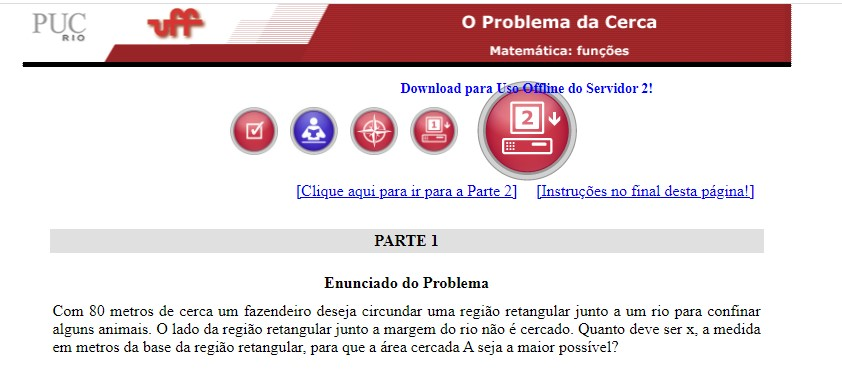
\includegraphics[width=\textwidth]{media/tec-print-servidor02.jpg}
    \caption{Botão ``Servidor 2", utilizado para baixar a cópia da atividade}
    \label{fig:serv02}
\end{figure}

\begin{figure}[hbt]
    \begin{subfigure}{0.5\textwidth}
    \centering
    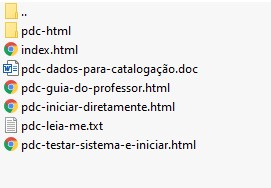
\includegraphics[width=.8\textwidth]{media/tec-pdc-zip.jpg}
    \caption{Todos os conteúdos do arquivo \texttt{pdc.zip}, com os conteúdos do módulo ``O Problema da Cerca"}
    \label{fig:pdc-zip}
    \end{subfigure}
    % 
    \hfill
    %  
    \begin{subfigure}{0.4\textwidth}
    \centering
    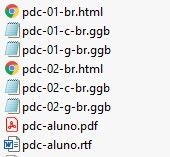
\includegraphics[width=.7\textwidth]{media/tec-pdc-html-alguns.jpg}
    \caption{Arquivos importantes dentro da pasta \texttt{pdc-html}, dentro da cópia do módulo ``O Problema da Cerca".}
    \label{fig:pdc-html}
    \end{subfigure}
    \caption{Imagens dos conteúdos do arquivo baixado do CDME.}
\end{figure}

\section{Obtendo o código de identificação de cada construção GeoGebra}

Ao longo do processo, descobrimos que o método que utilizaríamos para incorporar as construções em suas respectivas páginas exigia termos um código de identificação de cada atividade, que não estava presente na versão anterior do Projeto. Este código, é uma transcrição em formato \texttt{ggbBase64}\footnote{Um código em formato ggbBase64 é um texto composto de até 64 caracteres diferentes (base 64), que contém todas as informações de uma construção de maneira que a API do GeoGebra consiga decodificar.} das construções. Descobrimos que os códigos em ggbBase64 das construções podem ser gerados através do programa GeoGebra em sua versão ``3.2.46.11", exportando os arquivos como arquivos HTML, como mostrado na Figura~\ref{get-ggbBase64}.

\begin{figure}[htb]
    \centering
    
    \begin{subfigure}{\textwidth}
    \centering
    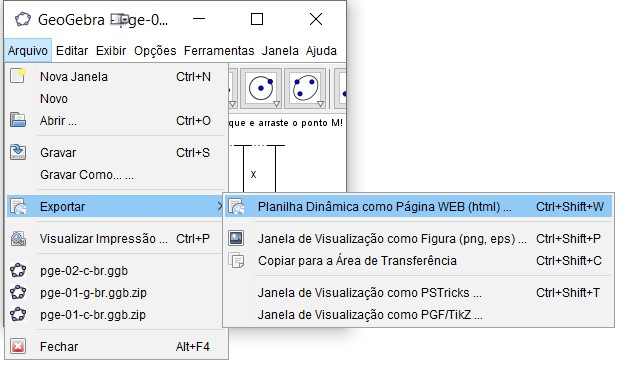
\includegraphics[width=0.7\textwidth]{media/tec-get-ggbBase64-01}
    \caption{Botão que abre a janela de exportação para html. Também pode ser usado o atalho Ctrl+Shift+W}
    \label{fig:getggb1}
    \end{subfigure}
    
    \begin{subfigure}{\textwidth}
    \centering
    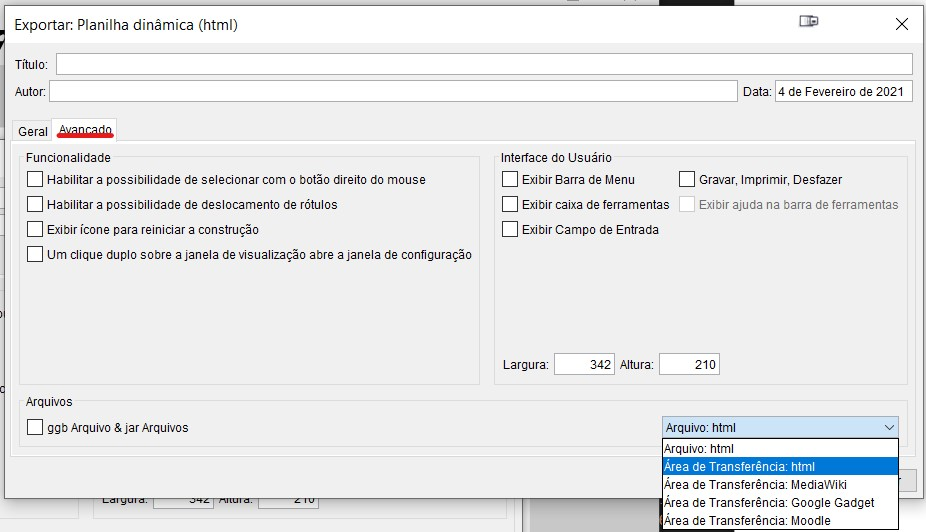
\includegraphics[width=0.9\textwidth]{media/tec-get-ggbBase64-02}
    \caption{A Janela de exportação do arquivo GeoGebra para html. Ambas as opções HTML te dão o mesmo texto, mas uma salva o arquivo no disco, e a outra simplesmente copia o texto para a área de transferência, onde pode ser colada em algum outro arquivo.}
    \label{fig:getggb2}
    \end{subfigure}
    \caption{Procedimento para obtenção do código de identificação ggbBase64 pelo programa \texttt{geogebra.jar}.}
    \label{get-ggbBase64}
\end{figure}

\begin{verbatim}
<applet name="ggbApplet" code="geogebra.GeoGebraApplet"
archive="geogebra.jar"
codebase="http://www.geogebra.org/webstart/3.2/unsigned/"
width="342" height="200" mayscript="true">
<param name="ggbBase64" value="{codigo-de-identificação}"/>
\end{verbatim}

Será gerado um único arquivo com extensão html. Este arquivo deve ser aberto com um editor de texto, e deve-se buscar o código de identificação dentro da tag como abaixo: 

O valor da o atributo \texttt{codigo-de-identificação} é a codificação em ggbBase64 da construção. Este valor é um texto muito longo. Outros parâmetros que serão úteis posteriormente são \texttt{width} e \texttt{height}, que nos informam, respectivamente, a largura e a altura, em pixels, da construção.

\section{Atualizando a página de atividade}

Com a identificação em mãos, a incorporação das construções se torna possível, introduzindo das seguintes linhas de código no lugar da antiga tag \texttt{<applet>}:

Abrindo a página da atividade (no nosso caso, a página ...) com um editor de texto, todo o conteúdo entre as tag \texttt{<applet>} e \texttt{</applet>}, incluindo estas tags, deve ser substituído pelas linhas abaixo:


\begin{verbatim}
    <script>
    var params_construct = {
          "id": "ggbApplet",
          "width":354,
          "height":214,
          "showMenuBar":false,
          "showAlgebraInput":false,
          "showToolBar":false,
          "showToolBarHelp":false,
          "showResetIcon":false,
          "enableLabelDrags":false,
          "enableShiftDragZoom":false,
          "enableRightClick":false,
          "errorDialogsActive":false,
          "useBrowserForJS":false,
          "ggbBase64": {codigo-de-identificação-obtido-na-seção-anterior}
          };
    params_construct.appletOnLoad = function(api) {
        /* ações necessárias mediante carregamento da construção */ };
    var construct_id = new GGBApplet("5.0", params_construc);
    window.addEventListener("load", function(){
        construct_id.inject("construct_id_container", "auto")});
    </script>
\end{verbatim}

O valor do campo \texttt{ggbBase64} de uma construção é o obtido a partir do seu respectivo arquivo .ggb, como descrito na seção anterior. Os valores de \texttt{width} e \texttt{height} podem ser os que foram obtidos naquela seção também, mas podem ser qualquer largura e altura convenientes.

As ações necessárias mediante carregamento já estavam bem definidas no código antigo, e aqui só foi necessário atualizar o método pelos quais eram chamadas.

\section{Adaptando o código para a API atual}

Após essas mudanças, as construções já devem estar operacionais na página, mas a programação que faz a comunicação dos applets com os botões e campos HTML ainda não deve estar funcionando, pois ainda estão na sintaxe utilizada pelos applets. Para sanar esse problema, temos que reescrever a maneira que as funções são chamadas no código.
\\

No modelo antigo, uma função \texttt{nome\_func}, de parâmetros \texttt{parametros\_func}  que interagia com o applet Java de uma construção \texttt{id\_construct} era chamada da seguinte maneira:

\begin{verbatim}
  document.getElementById("id_construct").nome_func(parametros_func);
\end{verbatim}

No GeoGebra para JavaScript, a mesma função, com os mesmos parâmetros e que interage com a mesma construção deve ser chamada da seguinte maneira:

\begin{verbatim}
    id_construct.nome_func(parametros_func);
\end{verbatim}

Essas mudanças podem ser feitas em qualquer editor de texto. Há alguns, como o Visual Studio Code, que possuem ferramentas para substituir todas as repetições de uma determinada sequência de caracteres\footnote{Conhecidas como \textit{strings} no mundo da informática.}

\section{Automatizando a atualização}

Todo o processo foi automatizado através de um \textit{script} em Python, disponível em repositório no GitHub, acessível em \url{https://github.com/fellipessanha/CDME-javascript/}, que fez as substituições como explicadas acima em todas as páginas.

O \textit{script} retira informações úteis --- como código de identificação ggbBase64, e opções como tornar a barra de menus inacessível --- de páginas HTML localizadas em uma pasta dentro do repositório, cria um código JavaScript que possibilita a inserção da construção na página da atividade, insere a atividade no lugar correto, e salva o código da página nova, com a codificação correta, em um arquivo separado, para evitar sobrescrever o código original.
\\

Para executar o código, basta executar o arquivo \texttt{conversion.py}, disponível no \href{https://github.com/fellipessanha/CDME-javascript/}{repositório}, com o Python, dentro do diretório da pasta que contém tanto as páginas que cujas construções devem ser convertidas, quanto a pasta com os respectivos códigos html das construções. No Windows, basta abrir o Prompt de Comando, navegar até a sua pasta destino --- \texttt{cd <pasta-destino>} --- e executar o comando ``\texttt{python conversion.py}". O programa atualiza com uma mensagem de texto para cada construção corretamente convertida.


\section{Módulos com construções tridimensionais}

Outro problema que se apresentou a nós foi o das construções tridimensionais, antes feitas com o software de visualização de figuras 3D JavaView. Ao contrário do GeoGebra, os desenvolvedores dessa biblioteca não disponibilizam nenhum tipo de suporte que nos permita converter as construções para implementação em HTML5, o que significa que tivemos que refazer todo o trabalho de visualização de figuras tridimensionais que correspondessem às situações propostas e, além de passarem no teste do arrastamento~\cite{de2020fases}, se comportassem como as já previamente utilizadas, além do esforço de formatação para encaixar o novo software no lugar do antigo..
\\

Escolhemos como ferramenta para solucionar o problema supracitado o próprio GeoGebra, que hoje em dia conta com suporte a janelas tridimensionais. Essa escolha tem a vantagem de padronizar todos os softwares do projeto facilitando qualquer tipo de manutenção futura no site, já que todas as construções terão funcionamentos similares.

Formatar as construções para que se encaixassem nos mesmos locais pré-definidos para os applets anteriores se mostrou a tarefa mais trabalhosa, visto que as construções eram muito diferentes entre si. A formatação foi feita ajeitando as figuras aos poucos, e testando o resultado na página do respectivo módulo.
\\

Além da formatação, foi necessário rodar alguns durante a inicialização da construção para garantir que o mouse se comportase como esperado, rotacionando a construção em torno de um eixo específico. O código utilizado é como o especificado abaixo:
\\

\begin{verbatim}
    var parameters3d ={
        "appletOnLoad":function(api){api.setMode(540);},
        /* variáveis necessárias para a construção */
    }
\end{verbatim}


Os conteúdos do parâmetro ``\texttt{appletOnLoad}" são os métodos executados pelo GeoGebra em sua inicialização, e o método especificado --- ``\texttt{api.setMode(540);}" --- serve para modificar a função do mouse na construção para alterar o ângulo da perspectiva da construção, ao invés da função original de interação com a figura.

% </script>
% <div id="lspApplet_container"></div>
% </td>
% <td align="center" bgcolor="#FFFFFF">
% <script>
%   var parameters = {
%   "id": "ggbApplet",
%   "width":354,
%   "height":214,
%   "showMenuBar":false,
%   "showAlgebraInput":false,
%   "showToolBar":false,
%   "customToolBar":"0 | 1 501 5 19 , 67 | 2 15 45 18 , 7 37 | 514 3 9 , 13 44 , 47 | 16 51 | 551 550 11 ,  20 22 21 23 , 55 56 57 , 12 | 69 | 510 511 , 512 513 | 533 531 , 534 532 , 522 523 , 537 536 , 535 , 538 | 521 520 | 36 , 38 49 560 | 571 30 29 570 31 33 | 17 | 540 40 41 42 , 27 28 35 , 6 , 502",
%   "showToolBarHelp":false,
%   "showResetIcon":false,
%   "enableLabelDrags":false,
%   "enableShiftDragZoom":false,
%   "enableRightClick":false,
%   "errorDialogsActive":false,
%   "useBrowserForJS":false,
%   "allowStyleBar":false,
%   "preventFocus":false,
%   "showZoomButtons":true,
%   "capturingThreshold":3,
%   // add code here to run when the applet starts
%   "appletOnLoad":function(api){ /* api.evalCommand('Segment((1,2),(3,4))');*/ },
%   "showFullscreenButton":false,
%   "scale":1,
%   "disableAutoScale":false,
%   "allowUpscale":false,
%   "clickToLoad":false,
%   "appName":"classic",
%   "showSuggestionButtons":false,
%   "buttonRounding":0.7,
%   "buttonShadows":false,
%   "language":"pt",
%   // use this instead of ggbBase64 to load a material from geogebra.org
%   // "material_id":"RHYH3UQ8",
%   // use this instead of ggbBase64 to load a .ggb file
%   // "filename":"myfile.ggb",
%   "ggbBase64": 'codigo=enorme'
%   };
%   // is3D=is 3D applet using 3D view, AV=Algebra View, SV=Spreadsheet View, CV=CAS View, EV2=Graphics View 2, CP=Construction Protocol, PC=Probability Calculator DA=Data Analysis, FI=Function Inspector, macro=Macros
%   var views = {'is3D': 1,'AV': 0,'SV': 0,'CV': 0,'EV2': 0,'CP': 0,'PC': 0,'DA': 0,'FI': 0,'macro': 0};
%   var applet = new GGBApplet(parameters, '5.0', views);
%   window.onload = function() {applet.inject('ggbApplet')};
%   applet.setPreviewImage('data:image/gif;base64,R0lGODlhAQABAAAAADs=','https://www.geogebra.org/images/GeoGebra_loading.png','https://www.geogebra.org/images/applet_play.png');
% //   ggbApplet.registerObjectUpdateListener('variavelX')
%   </script>